\section{Solution Description}

\subsection{Design Principles}

SPLA library is designed the way to maximize potential library performance, simplify its implementation and extensions, and to provided the end-user verbose, but effective interface allowing customization and precise control over operations execution. These ideas are captured in the following principles.

\begin{itemize}
    \item \textit{DAG-based expressions}. User constructs a computational expression from basic nodes and uses oriented edges to describe data dependencies between these nodes. 
    \item \textit{Automated hybrid-storage format}. Library uses internally specialized preprocessing to format data and automate its sharing between computational nodes.
    \item \textit{Automated scheduling}. Computational work is automatically scheduled between available threads and nodes for execution. Scheduling order, dependencies, and granularity are defined from DAG expression, submitted by a user.
    \item \textit{Customization of primitive types and operations}. Underlying primitives types and functions can be customized by user. The customization process does not require library re-compilation. 
    \item \textit{Exportable interface}. The library has a C++ interface with an automated reference-counting and with no-templates usage. It can be wrapped by C99 compatible API and exported to other languages, for example, in a form of a Python package.
\end{itemize}

\subsection{Architecture Overview}

Library general execution architecture is depicted in Fig.~\ref{fig:architecture}. As an input library accepts expression composed in the form of a DAG.
Nodes represent fundamental operations, such as vector-matrix multiplication. 
Links describe dependencies between nodes.
Expression execution is \textit{asynchronous}. 
User can block and wait until its completion, or without blocking probe the expression until it is either \textit{completed} or \textit{aborted}. 

Expression is transformed into a task graph. 
The task graph is submitted for execution to the task manager. 
Each task is processed by specialized \textit{NodeProcessor}, capable of processing a particular node type.
Each task, when executed, is split dynamically into a set of parallel sub-tasks. 
Each sub-task is processed by specialized \textit{Algorithm}, which is capable of processing input blocks of matrices or vectors in particular storage formats with a specific set of options. \textit{NodeProcessor} and \textit{Algorithm} are selected at runtime from a registry using properties and arguments of the expression. 
Thus, it allows precise processing and optimization of edge-cases.

The granularity level of sub-tasks is defined by the structure of underlying processed primitives. 
The target device for execution is automatically assigned for the sub-task based on expression and node parameters. 
Currently, the fixed assignment is supported.

\begin{figure}[t]
\centering
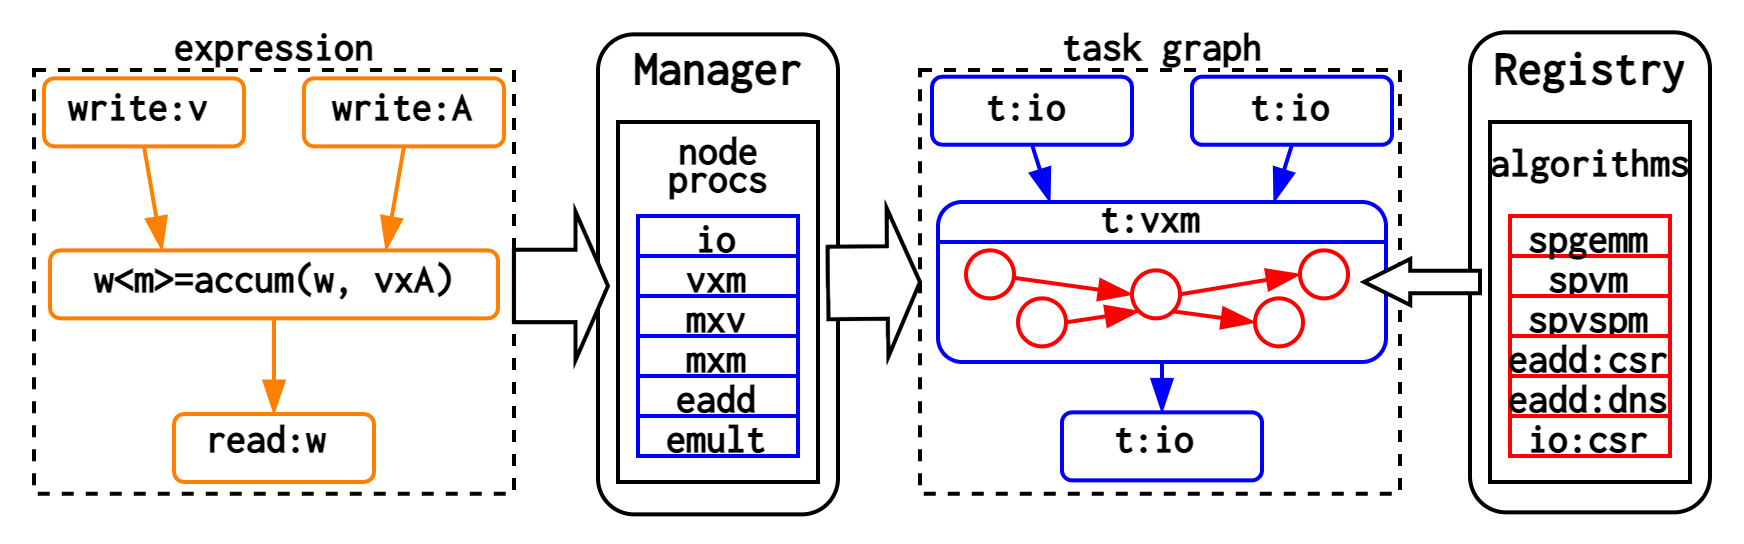
\includegraphics[width=0.95\linewidth]{architecture.png}
\caption{Library expression processing architecture.}
\label{fig:architecture}
\end{figure}
    
\subsection{Containers}

Library provides general \textit{M-by-N Matrix}, \textit{N Vector} and \textit{Scalar} data containers.
Underlying primitives types are specified by \textit{Type} object. 
Primitives are stored in a hybrid storage in a form of two- or one- dimensional blocks' grid for matrices and vectors respectively. 
Each block is empty (not stored) or stores some data in any format. Blocks are immutable, they can be safely shared across computational units.

Currently, COO/CSR blocks for matrices and COO/Dense blocks for vectors a are supported. Format choice is motivated by its simplicity and ease of implementation. 
Other formats, such as CSC, DCSR, ELL, etc., can be added to the library by the implementation of formats conversion or by the specialization of \textit{Algorithm} for a specific format.

\subsection{Algebraic Operations}

Library supports all commonly used linear algebra operations, such as \textit{mxm}, \textit{vxm}, \textit{eadd}, \textit{reduce}, \textit{transpose}. 
Other operations are coming soon since the library is still in development.
Interface of operations is designed \textit{similar} to GraphBLAS. 
It supports \textit{masking}, \textit{accum} of the result, \textit{add} and \textit{mult} user-functions specification, and \textit{descriptor} object for additional operation tweaking.

\subsection{Implementation Details}

Library uses OpenCL 1.2 as underlying compute API. 
Boost Compute~\cite{10.1145/2909437.2909454:boost:compute} is utilized as a high-level library on top of the OpenCL functionality. 
It provides thread-safe kernel caching, meta-kernel programming, and a set of basic parallel primitives such as \textit{device vector}, \textit{sort}, \textit{reduce}, \textit{scan}, etc., which is extended further to meet this project requirements.
Taskflow~\cite{Huang2022TaskflowAL} is used as a tasking library. It supports task-dependencies and dynamic tasking, utilized in order to create and execute sub-tasks. 

User-defined \textit{Types} are represented as POD-structures and handled by the library as fixed-size sequences of bytes.
User-defined \textit{Functions} are effectively textual strings with OpenCL code, injected into generalized meta-kernels.
Library has a number of predefined types, such as \textit{signed/unsigned integers}, \textit{floating point} types, and a set of common operations, such as \textit{arithmetic}, \textit{logic}, \textit{first/second}, etc.

For particular SpVSpM implementation ESC algorithm~\cite{10.1145/2699470:esc:algo} is employed. 
Masked SpGEMM is based on Yang et al. work~\cite{yang2019graphblast} solution. 
Tiled GPU merge path~\cite{inproceedings:gpu_merge_path} utilized for element-wise addition and masking implementation.
The code is generalized and written in a form of meta-kernels, so actual functions for elements reduction or multiplication are injected later.
Kernel compilation is done on demand if no previously cached entry is present.